% Options for packages loaded elsewhere
\PassOptionsToPackage{unicode}{hyperref}
\PassOptionsToPackage{hyphens}{url}
\PassOptionsToPackage{dvipsnames,svgnames*,x11names*}{xcolor}
%
\documentclass[
  ignorenonframetext,
]{beamer}
\usepackage{pgfpages}
\setbeamertemplate{caption}[numbered]
\setbeamertemplate{caption label separator}{: }
\setbeamercolor{caption name}{fg=normal text.fg}
\beamertemplatenavigationsymbolsempty
% Prevent slide breaks in the middle of a paragraph
\widowpenalties 1 10000
\raggedbottom
\setbeamertemplate{part page}{
  \centering
  \begin{beamercolorbox}[sep=16pt,center]{part title}
    \usebeamerfont{part title}\insertpart\par
  \end{beamercolorbox}
}
\setbeamertemplate{section page}{
  \centering
  \begin{beamercolorbox}[sep=12pt,center]{part title}
    \usebeamerfont{section title}\insertsection\par
  \end{beamercolorbox}
}
\setbeamertemplate{subsection page}{
  \centering
  \begin{beamercolorbox}[sep=8pt,center]{part title}
    \usebeamerfont{subsection title}\insertsubsection\par
  \end{beamercolorbox}
}
\AtBeginPart{
  \frame{\partpage}
}
\AtBeginSection{
  \ifbibliography
  \else
    \frame{\sectionpage}
  \fi
}
\AtBeginSubsection{
  \frame{\subsectionpage}
}
\usepackage{lmodern}
\usepackage{amssymb,amsmath}
\usepackage{ifxetex,ifluatex}
\ifnum 0\ifxetex 1\fi\ifluatex 1\fi=0 % if pdftex
  \usepackage[T1]{fontenc}
  \usepackage[utf8]{inputenc}
  \usepackage{textcomp} % provide euro and other symbols
\else % if luatex or xetex
  \usepackage{unicode-math}
  \defaultfontfeatures{Scale=MatchLowercase}
  \defaultfontfeatures[\rmfamily]{Ligatures=TeX,Scale=1}
\fi
% Use upquote if available, for straight quotes in verbatim environments
\IfFileExists{upquote.sty}{\usepackage{upquote}}{}
\IfFileExists{microtype.sty}{% use microtype if available
  \usepackage[]{microtype}
  \UseMicrotypeSet[protrusion]{basicmath} % disable protrusion for tt fonts
}{}
\makeatletter
\@ifundefined{KOMAClassName}{% if non-KOMA class
  \IfFileExists{parskip.sty}{%
    \usepackage{parskip}
  }{% else
    \setlength{\parindent}{0pt}
    \setlength{\parskip}{6pt plus 2pt minus 1pt}}
}{% if KOMA class
  \KOMAoptions{parskip=half}}
\makeatother
\usepackage{xcolor}
\IfFileExists{xurl.sty}{\usepackage{xurl}}{} % add URL line breaks if available
\IfFileExists{bookmark.sty}{\usepackage{bookmark}}{\usepackage{hyperref}}
\hypersetup{
  pdftitle={Dimension Reduction and Clustering},
  pdfauthor={Zack Treisman},
  colorlinks=true,
  linkcolor=Maroon,
  filecolor=Maroon,
  citecolor=blue,
  urlcolor=Blue,
  pdfcreator={LaTeX via pandoc}}
\urlstyle{same} % disable monospaced font for URLs
\newif\ifbibliography
\usepackage{color}
\usepackage{fancyvrb}
\newcommand{\VerbBar}{|}
\newcommand{\VERB}{\Verb[commandchars=\\\{\}]}
\DefineVerbatimEnvironment{Highlighting}{Verbatim}{commandchars=\\\{\}}
% Add ',fontsize=\small' for more characters per line
\usepackage{framed}
\definecolor{shadecolor}{RGB}{248,248,248}
\newenvironment{Shaded}{\begin{snugshade}}{\end{snugshade}}
\newcommand{\AlertTok}[1]{\textcolor[rgb]{0.94,0.16,0.16}{#1}}
\newcommand{\AnnotationTok}[1]{\textcolor[rgb]{0.56,0.35,0.01}{\textbf{\textit{#1}}}}
\newcommand{\AttributeTok}[1]{\textcolor[rgb]{0.77,0.63,0.00}{#1}}
\newcommand{\BaseNTok}[1]{\textcolor[rgb]{0.00,0.00,0.81}{#1}}
\newcommand{\BuiltInTok}[1]{#1}
\newcommand{\CharTok}[1]{\textcolor[rgb]{0.31,0.60,0.02}{#1}}
\newcommand{\CommentTok}[1]{\textcolor[rgb]{0.56,0.35,0.01}{\textit{#1}}}
\newcommand{\CommentVarTok}[1]{\textcolor[rgb]{0.56,0.35,0.01}{\textbf{\textit{#1}}}}
\newcommand{\ConstantTok}[1]{\textcolor[rgb]{0.00,0.00,0.00}{#1}}
\newcommand{\ControlFlowTok}[1]{\textcolor[rgb]{0.13,0.29,0.53}{\textbf{#1}}}
\newcommand{\DataTypeTok}[1]{\textcolor[rgb]{0.13,0.29,0.53}{#1}}
\newcommand{\DecValTok}[1]{\textcolor[rgb]{0.00,0.00,0.81}{#1}}
\newcommand{\DocumentationTok}[1]{\textcolor[rgb]{0.56,0.35,0.01}{\textbf{\textit{#1}}}}
\newcommand{\ErrorTok}[1]{\textcolor[rgb]{0.64,0.00,0.00}{\textbf{#1}}}
\newcommand{\ExtensionTok}[1]{#1}
\newcommand{\FloatTok}[1]{\textcolor[rgb]{0.00,0.00,0.81}{#1}}
\newcommand{\FunctionTok}[1]{\textcolor[rgb]{0.00,0.00,0.00}{#1}}
\newcommand{\ImportTok}[1]{#1}
\newcommand{\InformationTok}[1]{\textcolor[rgb]{0.56,0.35,0.01}{\textbf{\textit{#1}}}}
\newcommand{\KeywordTok}[1]{\textcolor[rgb]{0.13,0.29,0.53}{\textbf{#1}}}
\newcommand{\NormalTok}[1]{#1}
\newcommand{\OperatorTok}[1]{\textcolor[rgb]{0.81,0.36,0.00}{\textbf{#1}}}
\newcommand{\OtherTok}[1]{\textcolor[rgb]{0.56,0.35,0.01}{#1}}
\newcommand{\PreprocessorTok}[1]{\textcolor[rgb]{0.56,0.35,0.01}{\textit{#1}}}
\newcommand{\RegionMarkerTok}[1]{#1}
\newcommand{\SpecialCharTok}[1]{\textcolor[rgb]{0.00,0.00,0.00}{#1}}
\newcommand{\SpecialStringTok}[1]{\textcolor[rgb]{0.31,0.60,0.02}{#1}}
\newcommand{\StringTok}[1]{\textcolor[rgb]{0.31,0.60,0.02}{#1}}
\newcommand{\VariableTok}[1]{\textcolor[rgb]{0.00,0.00,0.00}{#1}}
\newcommand{\VerbatimStringTok}[1]{\textcolor[rgb]{0.31,0.60,0.02}{#1}}
\newcommand{\WarningTok}[1]{\textcolor[rgb]{0.56,0.35,0.01}{\textbf{\textit{#1}}}}
\usepackage{graphicx,grffile}
\makeatletter
\def\maxwidth{\ifdim\Gin@nat@width>\linewidth\linewidth\else\Gin@nat@width\fi}
\def\maxheight{\ifdim\Gin@nat@height>\textheight\textheight\else\Gin@nat@height\fi}
\makeatother
% Scale images if necessary, so that they will not overflow the page
% margins by default, and it is still possible to overwrite the defaults
% using explicit options in \includegraphics[width, height, ...]{}
\setkeys{Gin}{width=\maxwidth,height=\maxheight,keepaspectratio}
% Set default figure placement to htbp
\makeatletter
\def\fps@figure{htbp}
\makeatother
\setlength{\emergencystretch}{3em} % prevent overfull lines
\providecommand{\tightlist}{%
  \setlength{\itemsep}{0pt}\setlength{\parskip}{0pt}}
\setcounter{secnumdepth}{-\maxdimen} % remove section numbering

\pgfdeclareimage[width=3.5cm]{mcslogo}{../western_logo_hor_MCS_3C_pos.pdf}
\pgfdeclareimage[width=1cm]{ccbysa}{../ccbysa88x31.png}
\titlegraphic{\href{http://creativecommons.org/licenses/by-sa/4.0/}{\pgfuseimage{ccbysa}}
\hfill
\href{https://western.edu/program/mathematics/}{\pgfuseimage{mcslogo}}}
%\usecolortheme{wcu}
%\institute{Western Colorado University}
%\setbeamertemplate{navigation symbols}{}

\title{Dimension Reduction and Clustering}
\author{Zack Treisman}
\date{Spring 2021}

\begin{document}
\frame{\titlepage}

\begin{frame}[fragile]

\scriptsize

\begin{Shaded}
\begin{Highlighting}[]
\KeywordTok{library}\NormalTok{(ggplot2)}
\KeywordTok{library}\NormalTok{(dplyr)}
\KeywordTok{library}\NormalTok{(tidyr)}
\KeywordTok{library}\NormalTok{(vegan)}
\CommentTok{#library(devtools)}
\CommentTok{#install_github("ggbiplot")}
\CommentTok{#library(ggbiplot)}

\KeywordTok{set.seed}\NormalTok{(}\DecValTok{23}\NormalTok{)}
\end{Highlighting}
\end{Shaded}

\end{frame}

\begin{frame}{Philosophy}
\protect\hypertarget{philosophy}{}

There are many situations where we would like to discover structure in
data without explicitly specifying a predictor-response relationship
between variables. Generally, this means creating new variables out of
combinations of existing variables that provide more concise summaries.

\begin{itemize}
\tightlist
\item
  Data with correlated predictors or high dimension (many predictors)
  can be problematic.

  \begin{itemize}
  \tightlist
  \item
    Correlation leads to high variance in parameter estimates and
    significance levels.
  \item
    The curse of dimsionality (eg. \(1-0.9^{20}\approx0.89\)) means that
    high dimensional data are sparse, and statistical power is hard to
    come by.
  \end{itemize}
\item
  Reparameterizing may remove correlations and reduce dimension.
\end{itemize}

\end{frame}

\begin{frame}{Dimension Reduction}
\protect\hypertarget{dimension-reduction}{}

Variable selection is a \emph{supervised} technique for dimension
reduction (see also partial least squares), meaning that a response
variable guides the process.

\emph{Unsupervised} techniques create a set of new variables to replace
the existing ones. No response variable is specified in the algorithms.
Instead, we search for pattern within the predictors themselves. These
algorithms fall into two categories, according to the sort of variable
created.

\begin{itemize}
\tightlist
\item
  \textbf{Ordination} refers to tools that create new numeric variables.

  \begin{itemize}
  \tightlist
  \item
    PCA, NMDS, etc.
  \end{itemize}
\item
  Tools that perform \textbf{clustering} create new categorical
  variables.

  \begin{itemize}
  \tightlist
  \item
    \(K\)-means, hierarchical clustering.
  \end{itemize}
\end{itemize}

\end{frame}

\begin{frame}{Scaling and centering}
\protect\hypertarget{scaling-and-centering}{}

All of the methods that we'll discuss expect that all variables in the
data are either recorded on the same measurement scale or have been
rescaled so that the numerical ranges are comparable.

\begin{itemize}
\tightlist
\item
  Divide each variable by its standard deviation/(max-min)/IQR.
\item
  Centering is also a helpful thing to do. Subtract the mean of each
  variable from each observation, so that all variables have mean 0.
\end{itemize}

\end{frame}

\begin{frame}{\(K\)-means clustering}
\protect\hypertarget{k-means-clustering}{}

Suppose you have a set of numeric variables \(X=(X_1, \ldots, X_p)\),
and a collection of observations \(x_1, \ldots, x_n\), with
\(x_i=(x_{i1},\ldots,x_{ip})\).

\begin{enumerate}
\tightlist
\item
  Choose a positive integer \(K\). This is how many groups you plan to
  create in the data.
\item
  Randomly select points \(C_1, \ldots, C_K\) with coordinates in the
  range determined by the data.
\item
  For each observation \(x_i\), assign it to the group \(j\) for which
  the distance from \(x_i\) to the point \(C_j\) is the smallest.
\item
  For each group \(j\), compute the centroid of the observations in that
  group and replace \(C_j\) with this point.
\item
  Repeat steps 3 and 4 until no points change groups in step 3 or some
  predefined stopping criterion is met.
\end{enumerate}

\end{frame}

\begin{frame}[fragile]{\(K\)-means example}
\protect\hypertarget{k-means-example}{}

\scriptsize

\begin{Shaded}
\begin{Highlighting}[]
\NormalTok{x=}\KeywordTok{matrix}\NormalTok{(}\KeywordTok{rnorm}\NormalTok{(}\DecValTok{250}\OperatorTok{*}\DecValTok{2}\NormalTok{), }\DataTypeTok{ncol=}\DecValTok{2}\NormalTok{) }\CommentTok{# 250 random 2D points }
\NormalTok{x[}\DecValTok{1}\OperatorTok{:}\DecValTok{125}\NormalTok{,}\DecValTok{1}\NormalTok{]=x[}\DecValTok{1}\OperatorTok{:}\DecValTok{125}\NormalTok{,}\DecValTok{1}\NormalTok{]}\OperatorTok{+}\DecValTok{3}\NormalTok{; x[}\DecValTok{1}\OperatorTok{:}\DecValTok{125}\NormalTok{,}\DecValTok{2}\NormalTok{]=x[}\DecValTok{1}\OperatorTok{:}\DecValTok{125}\NormalTok{,}\DecValTok{2}\NormalTok{]}\OperatorTok{-}\DecValTok{4} \CommentTok{# Shift half right and down}
\NormalTok{km.out=}\KeywordTok{kmeans}\NormalTok{(x,}\DecValTok{2}\NormalTok{,}\DataTypeTok{nstart=}\DecValTok{20}\NormalTok{) }\CommentTok{# perform K-means with 2 clusters}
\KeywordTok{ggplot}\NormalTok{(}\KeywordTok{data.frame}\NormalTok{(x), }\KeywordTok{aes}\NormalTok{(X1, X2, }\DataTypeTok{color=}\KeywordTok{factor}\NormalTok{(km.out}\OperatorTok{$}\NormalTok{cluster))) }\OperatorTok{+}
\StringTok{    }\KeywordTok{geom_point}\NormalTok{()}\OperatorTok{+}\KeywordTok{labs}\NormalTok{(}\DataTypeTok{title=}\StringTok{"K-Means with K=2"}\NormalTok{, }\DataTypeTok{x=}\StringTok{""}\NormalTok{, }\DataTypeTok{y=}\StringTok{""}\NormalTok{, }\DataTypeTok{color=}\StringTok{"Cluster"}\NormalTok{)}
\end{Highlighting}
\end{Shaded}

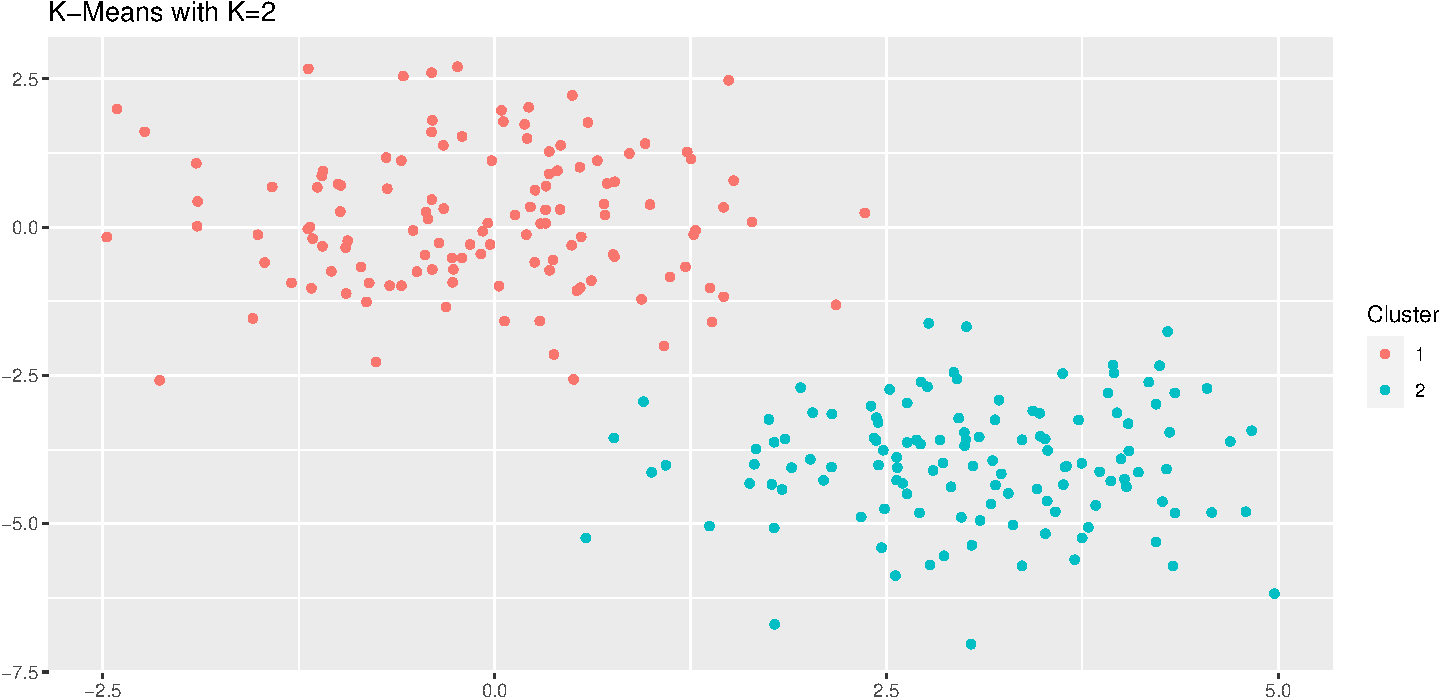
\includegraphics{unsupervised_learning_files/figure-beamer/unnamed-chunk-3-1.pdf}

\end{frame}

\begin{frame}[fragile]{\(K\)-means example (cont.)}
\protect\hypertarget{k-means-example-cont.}{}

\tiny

\begin{Shaded}
\begin{Highlighting}[]
\NormalTok{km.out}
\end{Highlighting}
\end{Shaded}

\begin{verbatim}
## K-means clustering with 2 clusters of sizes 125, 125
## 
## Cluster means:
##          [,1]       [,2]
## 1 -0.08315394  0.1278647
## 2  3.05729531 -3.9631181
## 
## Clustering vector:
##   [1] 2 2 2 2 2 2 2 2 2 2 2 2 2 2 2 2 2 2 2 2 2 2 2 2 2 2 2 2 2 2 2 2 2 2 2 2 2
##  [38] 2 2 2 2 2 2 2 2 2 2 2 2 2 2 2 2 2 2 2 2 2 2 2 2 2 2 2 2 2 2 2 2 2 2 2 2 2
##  [75] 2 2 2 2 2 2 2 2 2 2 2 2 2 2 2 2 2 2 2 2 2 2 2 2 2 2 2 2 2 2 2 2 2 2 2 2 2
## [112] 2 2 2 2 2 2 2 2 2 2 2 2 2 2 1 1 1 1 1 1 1 1 1 1 1 1 1 1 1 1 1 1 1 1 1 1 1
## [149] 1 1 1 1 1 1 1 1 1 1 1 1 1 1 1 1 1 1 1 1 1 1 1 1 1 1 1 1 1 1 1 1 1 1 1 1 1
## [186] 1 1 1 1 1 1 1 1 1 1 1 1 1 1 1 1 1 1 1 1 1 1 1 1 1 1 1 1 1 1 1 1 1 1 1 1 1
## [223] 1 1 1 1 1 1 1 1 1 1 1 1 1 1 1 1 1 1 1 1 1 1 1 1 1 1 1 1
## 
## Within cluster sum of squares by cluster:
## [1] 280.3319 232.1237
##  (between_SS / total_SS =  76.4 %)
## 
## Available components:
## 
## [1] "cluster"      "centers"      "totss"        "withinss"     "tot.withinss"
## [6] "betweenss"    "size"         "iter"         "ifault"
\end{verbatim}

\end{frame}

\begin{frame}[fragile]{The number of clusters is a parameter to choose}
\protect\hypertarget{the-number-of-clusters-is-a-parameter-to-choose}{}

\scriptsize

\begin{Shaded}
\begin{Highlighting}[]
\NormalTok{km.out=}\KeywordTok{kmeans}\NormalTok{(x,}\DecValTok{3}\NormalTok{,}\DataTypeTok{nstart=}\DecValTok{20}\NormalTok{)}
\end{Highlighting}
\end{Shaded}

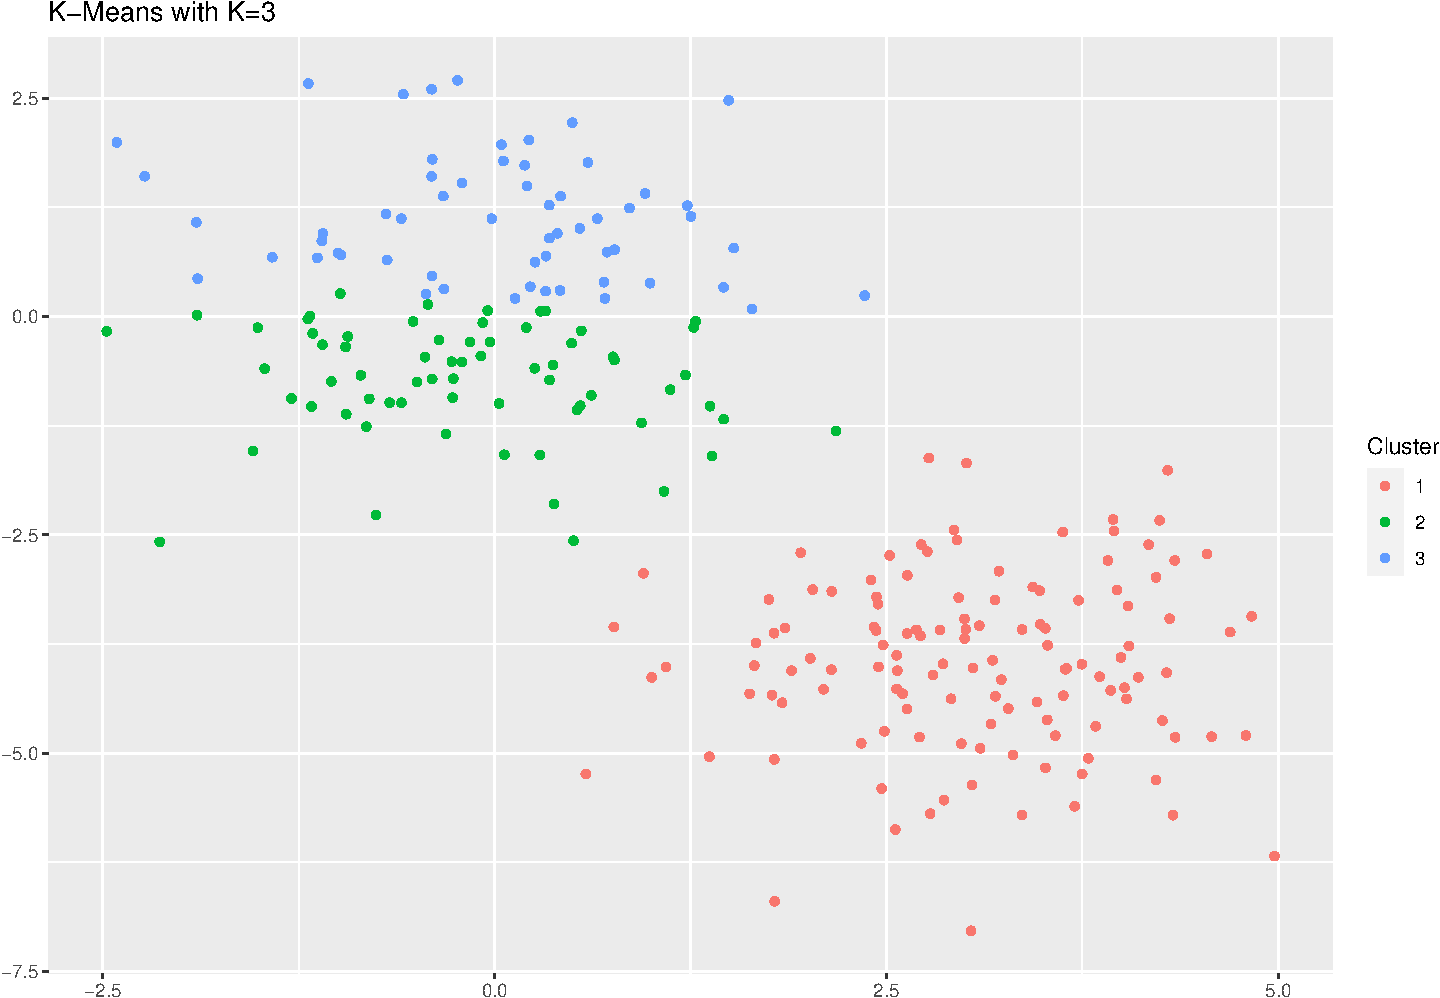
\includegraphics{unsupervised_learning_files/figure-beamer/unnamed-chunk-6-1.pdf}

\end{frame}

\begin{frame}[fragile]{Another parameter is how many times to restart
the algorithm}
\protect\hypertarget{another-parameter-is-how-many-times-to-restart-the-algorithm}{}

A bad initial choice of \(C_1 \ldots C_K\) can lead the algorithm to a
local minimum that's not optimal.

\begin{Shaded}
\begin{Highlighting}[]
\KeywordTok{set.seed}\NormalTok{(}\DecValTok{1}\NormalTok{)}
\NormalTok{km.out=}\KeywordTok{kmeans}\NormalTok{(x,}\DecValTok{5}\NormalTok{,}\DataTypeTok{nstart=}\DecValTok{1}\NormalTok{)}
\NormalTok{km.out}\OperatorTok{$}\NormalTok{tot.withinss}
\end{Highlighting}
\end{Shaded}

\begin{verbatim}
## [1] 317.9313
\end{verbatim}

\begin{Shaded}
\begin{Highlighting}[]
\NormalTok{km.out=}\KeywordTok{kmeans}\NormalTok{(x,}\DecValTok{5}\NormalTok{,}\DataTypeTok{nstart=}\DecValTok{20}\NormalTok{)}
\NormalTok{km.out}\OperatorTok{$}\NormalTok{tot.withinss}
\end{Highlighting}
\end{Shaded}

\begin{verbatim}
## [1] 268.3861
\end{verbatim}

\end{frame}

\begin{frame}[fragile]{Extensions and other considerations}
\protect\hypertarget{extensions-and-other-considerations}{}

\begin{itemize}
\tightlist
\item
  \(K\)-means-like algorithms with other notions of distance can be done
  with the \texttt{flexclust} package.
\item
  Data that change multiplicatively (eg. percentages) should perhaps be
  log transformed first.
\item
  When plotting clusters in high dimensional data, it may not be
  possible to see the separation in a plot of only two dimensions.
\end{itemize}

\end{frame}

\begin{frame}{Hierarchical clustering}
\protect\hypertarget{hierarchical-clustering}{}

A totally different method of clustering is \emph{hierarchical
clustering}

\begin{enumerate}
\tightlist
\item
  Each observation starts in its own cluster.
\item
  Pairwise distances between clusters are computed.
\item
  The two closest clusters are merged.
\item
  Repeat steps 2 and 3 until all observations are in one cluster.
\item
  The resulting tree of merging clusters can be cut at various levels to
  give set numbers of clusters.
\end{enumerate}

There are many ways to compute the distances in step 2.

\end{frame}

\begin{frame}[fragile]{West Fork Fire Complex Data}
\protect\hypertarget{west-fork-fire-complex-data}{}

This is a project I'm working on with Jonathan Coop. We're looking at
vegetation data from sites in the San Juans recovering from impacts of
beetles and fire.

\scriptsize

\begin{Shaded}
\begin{Highlighting}[]
\NormalTok{veg_data <-}\StringTok{ }\KeywordTok{read.csv}\NormalTok{(}\StringTok{"data/West_Fork_Plants.csv"}\NormalTok{)}
\KeywordTok{set.seed}\NormalTok{(}\DecValTok{1}\NormalTok{)}
\KeywordTok{sample_n}\NormalTok{(veg_data,}\DecValTok{10}\NormalTok{)[}\DecValTok{1}\OperatorTok{:}\DecValTok{8}\NormalTok{]}
\end{Highlighting}
\end{Shaded}

\begin{verbatim}
##       Plot_ID     Type  Code Stratum Cover Height      Genus      Species
## 1    F_24_720   Burned ASAL7       5   0.5    0.1 Astragalus      alpinus
## 2   F_14_5080   Burned POGR9       5   0.1    0.1 Potentilla     gracilis
## 3   F_14_8494   Burned DAPA2       5   2.5    0.5  Danthonia       parryi
## 4   N_31_5843 Unburned POPU3       5   0.5    0.2 Polemonium   pulchellum
## 5   F_24_4594   Burned CARO5       5   2.5    0.2      Carex       rossii
## 6   N_14_9086 Unburned  PIEN       2  17.5    3.0      Picea  engelmannii
## 7   F_33_3456   Burned ELTR7       5   0.5    0.6     Elymus trachycaulus
## 8   N_41_5768 Unburned  ABLA       2   2.5    3.5      Abies   lasiocarpa
## 9  N_41_10975 Unburned  OSDE       5   2.5    0.5  Osmorhiza  depauperata
## 10 N_34_11403 Unburned POTR5       3   0.1    1.0    Populus  tremuloides
\end{verbatim}

\end{frame}

\begin{frame}[fragile]{Pivot Wider}
\protect\hypertarget{pivot-wider}{}

Create a data matrix where the rows are sites and the columns are
species, with the entries percent cover for that species at that site.

\scriptsize

\begin{Shaded}
\begin{Highlighting}[]
\NormalTok{spp_cov<-}\KeywordTok{as_tibble}\NormalTok{(veg_data[}\KeywordTok{c}\NormalTok{(}\StringTok{"Plot_ID"}\NormalTok{, }\StringTok{"Code"}\NormalTok{, }\StringTok{"Cover"}\NormalTok{)])}
\NormalTok{spp_cov<-}\KeywordTok{with}\NormalTok{(spp_cov, spp_cov[}\KeywordTok{order}\NormalTok{(spp_cov}\OperatorTok{$}\NormalTok{Code), ])}
\NormalTok{spp_cov<-spp_cov[}\OperatorTok{!}\NormalTok{(spp_cov}\OperatorTok{$}\NormalTok{Code }\OperatorTok{==}\StringTok{ "Unknown"}\NormalTok{),] }\CommentTok{# get rid of unknowns}
\NormalTok{spp_cov_matrix<-spp_cov }\OperatorTok\StringTok{ }\KeywordTok{pivot_wider}\NormalTok{(}\DataTypeTok{names_from =}\NormalTok{ Code, }
                                        \DataTypeTok{values_from =}\NormalTok{ Cover,}
                                        \DataTypeTok{values_fn =}\NormalTok{ sum)}
\NormalTok{spp_cov_matrix[}\KeywordTok{is.na}\NormalTok{(spp_cov_matrix)] <-}\StringTok{ }\DecValTok{0} \CommentTok{# zeros instead of NAs}
\KeywordTok{head}\NormalTok{(spp_cov_matrix[,}\DecValTok{1}\OperatorTok{:}\DecValTok{10}\NormalTok{],}\DecValTok{10}\NormalTok{)}
\end{Highlighting}
\end{Shaded}

\begin{verbatim}
## # A tibble: 10 x 10
##    Plot_ID     ABCO  ABLA ACCO4  ACGL ACMI2 ACRU2  ADMO  ADPE AGAU2
##    <chr>      <dbl> <dbl> <dbl> <dbl> <dbl> <dbl> <dbl> <dbl> <dbl>
##  1 F_14_6810   17.5  49       0   0     0.1     0     0     0   0  
##  2 F_32_9673    2.5   3       0   2.5   0       0     0     0   0  
##  3 F_13_4275    0    39       0   0     0       0     0     0   0  
##  4 F_13_6435    0     0.5     0   0     0.5     0     0     0   0  
##  5 F_14_4273    0     0.1     0   0     0       0     0     0   0  
##  6 F_14_4283    0    51.5     0   0     0       0     0     0   0  
##  7 F_14_9251    0    12.5     0   0     0       0     0     0   0  
##  8 F_22_10708   0    18.5     0   0     0       0     0     0   0.1
##  9 F_22_9346    0     7.5     0   0     0       0     0     0   0  
## 10 F_23_3312    0    10       0   0     0       0     0     0   0
\end{verbatim}

\end{frame}

\begin{frame}[fragile]{Compute the tree}
\protect\hypertarget{compute-the-tree}{}

Use Bray-Curtis dissimilarity to measure ``distance'' between clusters.
\scriptsize

\begin{Shaded}
\begin{Highlighting}[]
\NormalTok{bc_diss <-}\StringTok{ }\KeywordTok{vegdist}\NormalTok{(spp_cov_matrix[,}\OperatorTok{-}\DecValTok{1}\NormalTok{],}\StringTok{"bray"}\NormalTok{)}
\NormalTok{diss_mat <-}\StringTok{ }\KeywordTok{as.matrix}\NormalTok{(bc_diss)}
\NormalTok{bc_tree <-}\StringTok{ }\KeywordTok{hclust}\NormalTok{(bc_diss)}
\KeywordTok{plot}\NormalTok{(bc_tree)}
\end{Highlighting}
\end{Shaded}

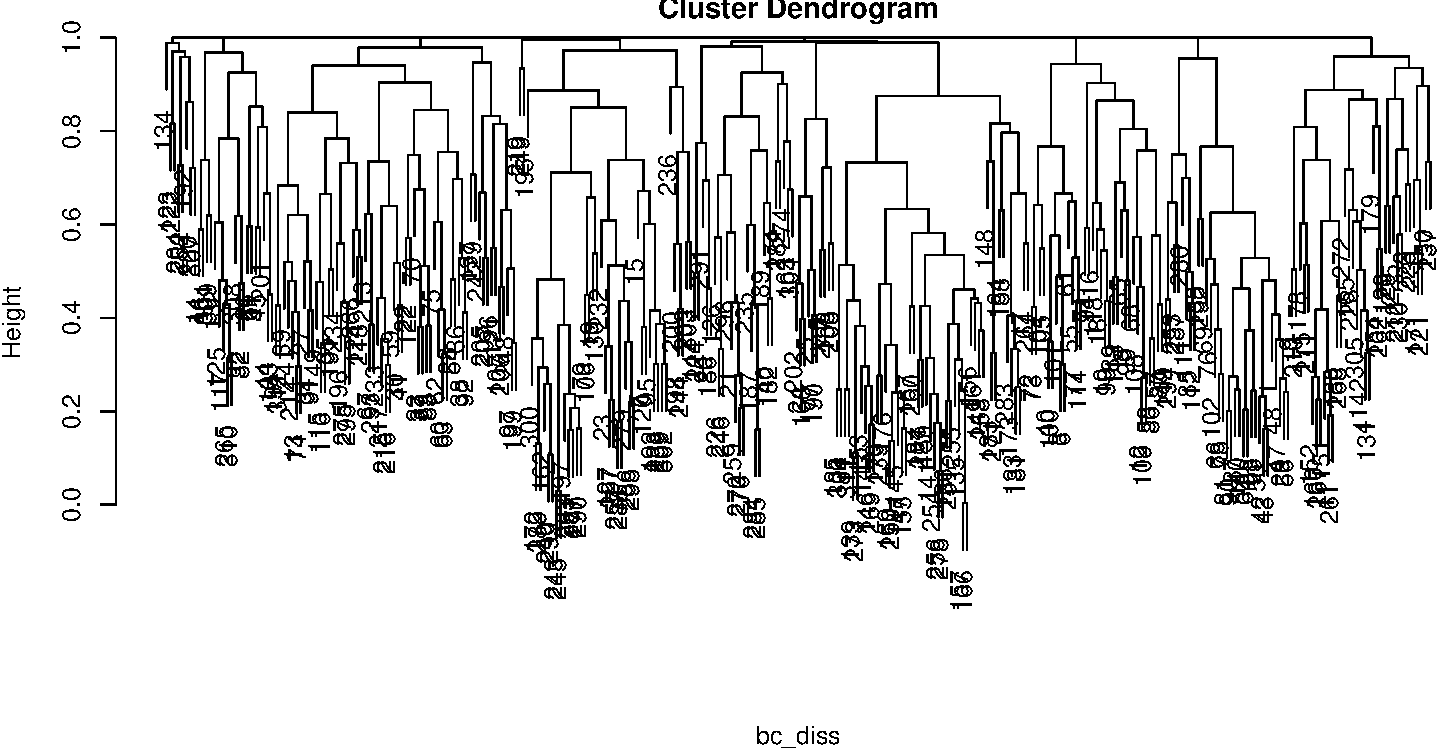
\includegraphics{unsupervised_learning_files/figure-beamer/unnamed-chunk-10-1.pdf}

\end{frame}

\begin{frame}[fragile]{Determine optimal number of clusters (scree
plot)}
\protect\hypertarget{determine-optimal-number-of-clusters-scree-plot}{}

Devise a metric of the information in the clustering and compute it as
you vary \(K\).

\scriptsize

\begin{Shaded}
\begin{Highlighting}[]
\NormalTok{k.max<-}\DecValTok{20}
\NormalTok{dpc <-}\StringTok{ }\KeywordTok{sapply}\NormalTok{(}\DecValTok{1}\OperatorTok{:}\NormalTok{k.max, }\ControlFlowTok{function}\NormalTok{(k)\{}
\NormalTok{    bc<-}\KeywordTok{cutree}\NormalTok{(bc_tree, k)}
    \KeywordTok{sum}\NormalTok{(}\KeywordTok{sapply}\NormalTok{(}\DecValTok{1}\OperatorTok{:}\NormalTok{k, }\ControlFlowTok{function}\NormalTok{(x) }\KeywordTok{sum}\NormalTok{(diss_mat[bc}\OperatorTok{==}\NormalTok{x,bc}\OperatorTok{==}\NormalTok{x]) )) }
\NormalTok{  \} )}
\end{Highlighting}
\end{Shaded}

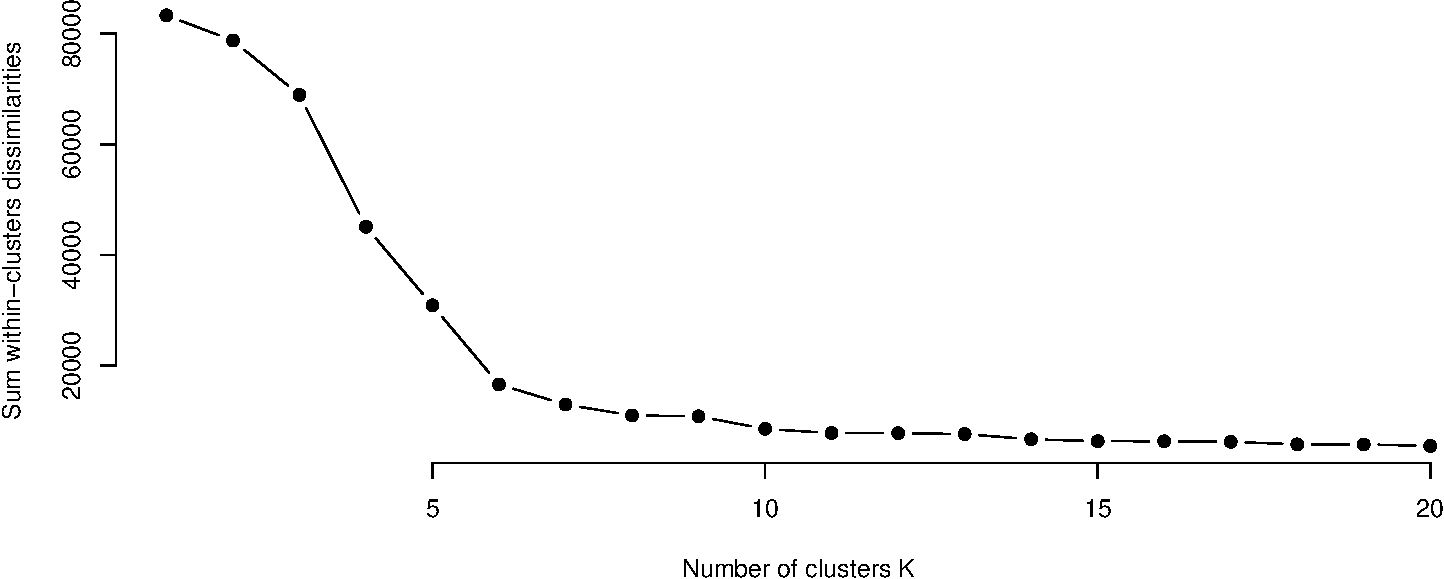
\includegraphics{unsupervised_learning_files/figure-beamer/unnamed-chunk-12-1.pdf}
\normalsize

There's an elbow at 6 clusters, so that's \(K\). \scriptsize

\begin{Shaded}
\begin{Highlighting}[]
\NormalTok{bc6<-}\KeywordTok{cutree}\NormalTok{(bc_tree, }\DataTypeTok{k=}\DecValTok{6}\NormalTok{)}
\end{Highlighting}
\end{Shaded}

\end{frame}

\begin{frame}[fragile]{Interpreting the clusters}
\protect\hypertarget{interpreting-the-clusters}{}

\scriptsize

\begin{Shaded}
\begin{Highlighting}[]
\NormalTok{plot_groups <-}\StringTok{ }\KeywordTok{tibble}\NormalTok{(}\DataTypeTok{Plot_ID =}\NormalTok{ spp_cov_matrix}\OperatorTok{$}\NormalTok{Plot_ID, }\DataTypeTok{bc_6 =}\NormalTok{ bc6)}
\NormalTok{plot_groups}\OperatorTok{$}\NormalTok{bc_}\DecValTok{6}\NormalTok{ <-}\StringTok{ }\KeywordTok{factor}\NormalTok{(plot_groups}\OperatorTok{$}\NormalTok{bc_}\DecValTok{6}\NormalTok{)}
\NormalTok{veg_data <-}\StringTok{ }\KeywordTok{merge}\NormalTok{(veg_data, plot_groups)}
\NormalTok{west_fork_trees <-}\StringTok{ }\KeywordTok{droplevels}\NormalTok{(veg_data[veg_data}\OperatorTok{$}\NormalTok{LifeForm}\OperatorTok{==}\StringTok{"Tree"}\NormalTok{, ])}
\NormalTok{west_fork_trees}\OperatorTok{$}\NormalTok{Form <-}\StringTok{ }\KeywordTok{factor}\NormalTok{(}\KeywordTok{ifelse}\NormalTok{(}\KeywordTok{grepl}\NormalTok{(}\StringTok{"POTR"}\NormalTok{,west_fork_trees}\OperatorTok{$}\NormalTok{Code),}
                                      \StringTok{"aspen"}\NormalTok{, }\StringTok{"conifer"}\NormalTok{))}
\end{Highlighting}
\end{Shaded}

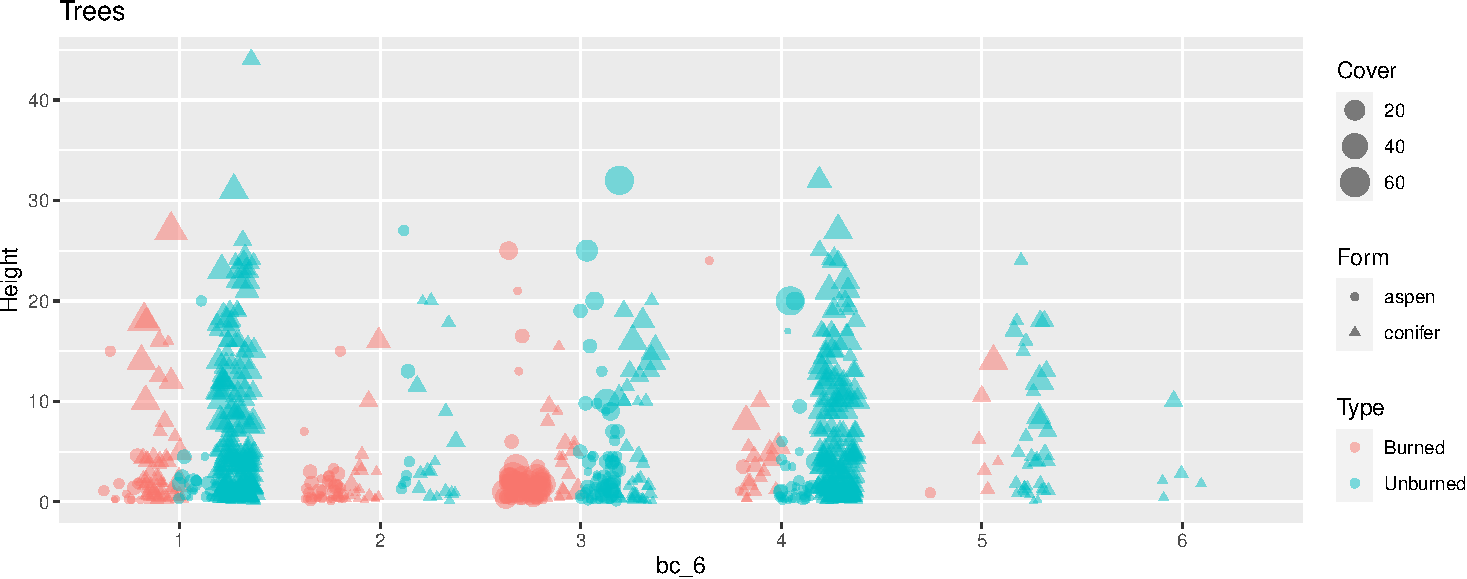
\includegraphics{unsupervised_learning_files/figure-beamer/unnamed-chunk-15-1.pdf}
\normalsize Having created this variable, it remains to determine what
it means.

\end{frame}

\begin{frame}{Geographic distribution of the groups}
\protect\hypertarget{geographic-distribution-of-the-groups}{}

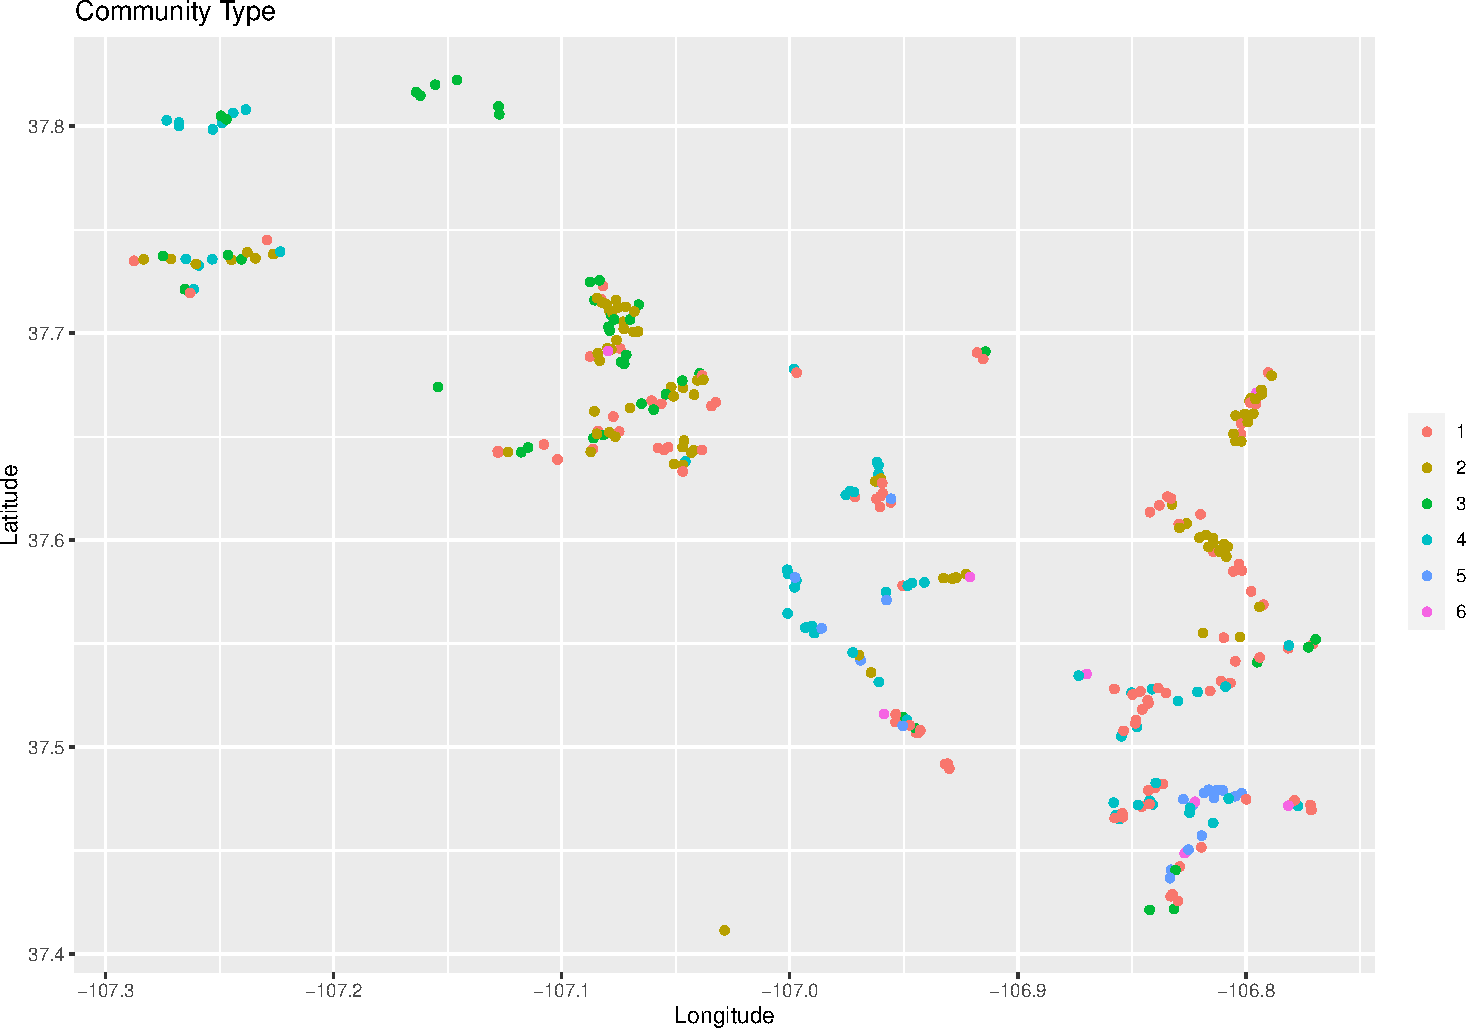
\includegraphics{unsupervised_learning_files/figure-beamer/unnamed-chunk-16-1.pdf}

\end{frame}

\begin{frame}[fragile]{What plants make up the communities?}
\protect\hypertarget{what-plants-make-up-the-communities}{}

We might be interested in what plants are specific to each community.
\scriptsize

\begin{Shaded}
\begin{Highlighting}[]
\NormalTok{get_codes <-}\StringTok{ }\ControlFlowTok{function}\NormalTok{(x)}\KeywordTok{unique}\NormalTok{(veg_data[veg_data}\OperatorTok{$}\NormalTok{bc_}\DecValTok{6}\OperatorTok{==}\NormalTok{x,]}\OperatorTok{$}\NormalTok{Code)}
\NormalTok{only_here <-}\StringTok{ }
\StringTok{    }\ControlFlowTok{function}\NormalTok{(x) \{}
\NormalTok{    onlyX <-}\StringTok{ }\KeywordTok{get_codes}\NormalTok{(x)}
    \ControlFlowTok{for}\NormalTok{(i }\ControlFlowTok{in} \KeywordTok{setdiff}\NormalTok{(}\DecValTok{1}\OperatorTok{:}\DecValTok{6}\NormalTok{,x)) \{onlyX <-}\StringTok{ }\KeywordTok{setdiff}\NormalTok{(onlyX, }\KeywordTok{get_codes}\NormalTok{(i))\}}
\NormalTok{    onlyX\}}
\KeywordTok{only_here}\NormalTok{(}\DecValTok{1}\NormalTok{)}
\end{Highlighting}
\end{Shaded}

\begin{verbatim}
##  [1] "VACE"   "ABCO"   "CHDE2"  "EPHA"   "PECR5"  "ANMI3"  "ARMI4"  "SOSC2" 
##  [9] "MIGU"   "JUEN"   "CAAU3"  "SIDR"   "BOGR2"  "VAAT2"  "LICO6"  "COMA25"
## [17] "POBI6"  "GEPA"   "PIPO"   "PONE2"  "HEQU2"  "FESO"   "DRRE"   "MARE"  
## [25] "FRSP"   "CARU"
\end{verbatim}

\begin{Shaded}
\begin{Highlighting}[]
\KeywordTok{only_here}\NormalTok{(}\DecValTok{2}\NormalTok{)}
\end{Highlighting}
\end{Shaded}

\begin{verbatim}
##  [1] "ARCA13" "AGEX"   "JUME3"  "ROBL"   "HECO26" "CICL"   "DYGR"   "FEBR"  
##  [9] "PIPU9"  "MELA2"  "PONEI2"
\end{verbatim}

\end{frame}

\begin{frame}[fragile]{What plants are most common in each community?}
\protect\hypertarget{what-plants-are-most-common-in-each-community}{}

\scriptsize

\begin{Shaded}
\begin{Highlighting}[]
\NormalTok{group_summary_plants <-}\StringTok{ }\NormalTok{veg_data }\OperatorTok\StringTok{ }\NormalTok{dplyr}\OperatorTok{::}\KeywordTok{group_by}\NormalTok{(bc_}\DecValTok{6}\NormalTok{) }\OperatorTok
\StringTok{  }\NormalTok{dplyr}\OperatorTok{::}\KeywordTok{summarise}\NormalTok{(}\DataTypeTok{num_sites =} \KeywordTok{length}\NormalTok{(}\KeywordTok{unique}\NormalTok{(Plot_ID)), }
            \DataTypeTok{num_species =} \KeywordTok{length}\NormalTok{(}\KeywordTok{unique}\NormalTok{(Code)),}
            \DataTypeTok{burn_prop =} \KeywordTok{sum}\NormalTok{(Type}\OperatorTok{==}\StringTok{"Burned"}\NormalTok{)}\OperatorTok{/}\NormalTok{num_sites,}
            \DataTypeTok{most_com =} \KeywordTok{tail}\NormalTok{(}\KeywordTok{names}\NormalTok{(}\KeywordTok{sort}\NormalTok{(}\KeywordTok{table}\NormalTok{(Code))), }\DecValTok{1}\NormalTok{),}
            \DataTypeTok{second_com =} \KeywordTok{tail}\NormalTok{(}\KeywordTok{names}\NormalTok{(}\KeywordTok{sort}\NormalTok{(}\KeywordTok{table}\NormalTok{(Code))), }\DecValTok{2}\NormalTok{)[}\DecValTok{1}\NormalTok{],}
            \DataTypeTok{third_com =} \KeywordTok{tail}\NormalTok{(}\KeywordTok{names}\NormalTok{(}\KeywordTok{sort}\NormalTok{(}\KeywordTok{table}\NormalTok{(Code))), }\DecValTok{3}\NormalTok{)[}\DecValTok{1}\NormalTok{])}
\NormalTok{group_summary_plants}
\end{Highlighting}
\end{Shaded}

\begin{verbatim}
## # A tibble: 6 x 7
##   bc_6  num_sites num_species burn_prop most_com second_com third_com
##   <fct>     <int>       <int>     <dbl> <chr>    <chr>      <chr>    
## 1 1            99         229      9.24 ABLA     PIEN       CHAN9    
## 2 2            83         175     16.6  TAOF     CASI12     CHAN9    
## 3 3            43         152     11.1  POTR5    CHAN9      TAOF     
## 4 4            60         210      2.15 PIEN     ABLA       FRVI     
## 5 5            19         112      5.79 PIEN     ABLA       BRCI2    
## 6 6             8          95     15.8  TRSP2    POPR       RIMO2
\end{verbatim}

\end{frame}

\begin{frame}{Ordination}
\protect\hypertarget{ordination}{}

With the data that are correlated rather than clustered, the goal is to
find a new set of directions in which the data are uncorrelated.

\begin{itemize}
\tightlist
\item
  Ordination produces a low-dimensional representation of a dataset. It
  finds a sequence of combinations of the variables that have maximal
  variance, and are mutually uncorrelated.
\item
  Apart from producing derived variables for use in supervised learning
  problems, ordination also serves as a tool for data visualization. For
  example, this is useful after clustering for plotting and interpreting
  results.
\end{itemize}

\end{frame}

\begin{frame}{Principal Components Analysis (PCA)}
\protect\hypertarget{principal-components-analysis-pca}{}

Here, I am closely following James et al. (2013).

\begin{itemize}
\item
  The \emph{first principal component} of a set of features
  \(X_1, X_2,\ldots, X_p\) is the normalized linear combination \[
  Z_1 = \phi_{11} X_1 + \phi_{21} X_2 + \cdots + \phi_{p1} X_p
  \] that has the largest variance. By \emph{normalized}, we mean that
  \(\sum_{j=1}^p \phi_{j1} = 1\).
\item
  We refer to the elements \(\phi_{11}, \ldots , \phi_{p1}\) as the
  loadings of the first principal component; together, the loadings make
  up the principal component loading vector,
  \(\phi_1 = (\phi_{11} \phi_{21} \ldots \phi_{p1} )^t\).
\item
  The second principal component is the linear combination of
  \(X_1, X_2,\ldots, X_p\) that has maximal variance among all linear
  combinations that are uncorrelated with \(Z_1\).
\item
  Further principal components are defined similarly.
\end{itemize}

\end{frame}

\begin{frame}{Computation of principal components}
\protect\hypertarget{computation-of-principal-components}{}

To compute the principal components, continuing with the notation from
above, the data are a matrix \(M=[x_{ij}]\) where \(i\) denotes the
observation and \(j\) the variable. Assume that the column means are
zero (data are centered).

\begin{itemize}
\tightlist
\item
  The \emph{singular value decomposition} factors the matrix into
  \(M=U\Sigma V^t\) where \(U\) and \(V\) are orthogonal and \(\Sigma\)
  is diagonal.
\item
  The columns of \(V\) are called the \textbf{principal directions}.
\item
  The columns of \(U\Sigma\) are the \textbf{principal components}
\end{itemize}

The details of this computation are probably not important, but in order
to understand what is going on with ordination in general, it is useful
to think in terms of linear algebra.

\end{frame}

\begin{frame}[fragile]{PCA example}
\protect\hypertarget{pca-example}{}

The plot of the observations and the variables on the axes defined by
the principal components is called a biplot.

\scriptsize

\begin{Shaded}
\begin{Highlighting}[]
\NormalTok{pca.climate <-}\StringTok{ }\KeywordTok{prcomp}\NormalTok{(climate71_}\DecValTok{00}\NormalTok{[,}\OperatorTok{-}\KeywordTok{c}\NormalTok{(}\DecValTok{1}\OperatorTok{:}\DecValTok{5}\NormalTok{,}\DecValTok{29}\NormalTok{)], }\DataTypeTok{scale =} \OtherTok{TRUE}\NormalTok{)}
\KeywordTok{library}\NormalTok{(ggbiplot) }\CommentTok{# library(devtools); install_github("ggbiplot")}
\KeywordTok{ggbiplot}\NormalTok{(pca.climate, }\DataTypeTok{obs.scale =} \DecValTok{1}\NormalTok{, }\DataTypeTok{var.scale =} \DecValTok{1}\NormalTok{, }\DataTypeTok{circle =} \OtherTok{TRUE}\NormalTok{,}
         \DataTypeTok{groups =}\NormalTok{ climate71_}\DecValTok{00}\OperatorTok{$}\NormalTok{bc_}\DecValTok{6}\NormalTok{) }\OperatorTok{+}\StringTok{ }\KeywordTok{theme}\NormalTok{(}\DataTypeTok{text =} \KeywordTok{element_text}\NormalTok{(}\DataTypeTok{size =} \DecValTok{8}\NormalTok{))}
\end{Highlighting}
\end{Shaded}

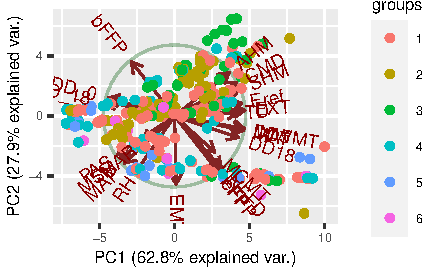
\includegraphics{unsupervised_learning_files/figure-beamer/fig.-1.pdf}

\end{frame}

\begin{frame}[fragile]{Interpreting the components}
\protect\hypertarget{interpreting-the-components}{}

When working with PCA, we are often most interested in the loadings
(representations of the features in terms of the principal components)
\scriptsize

\begin{Shaded}
\begin{Highlighting}[]
\NormalTok{climate_basis <-}\StringTok{ }\NormalTok{pca.climate}\OperatorTok{$}\NormalTok{rotation}
\NormalTok{climate_basis[}\DecValTok{1}\OperatorTok{:}\DecValTok{5}\NormalTok{,}\DecValTok{1}\OperatorTok{:}\DecValTok{3}\NormalTok{]}
\end{Highlighting}
\end{Shaded}

\begin{verbatim}
##             PC1         PC2         PC3
## MAT   0.2562305 -0.08088240  0.04614361
## MWMT  0.2575102 -0.06975190 -0.08307110
## MCMT  0.1485913 -0.20112174  0.59966061
## TD    0.2353614  0.01881473 -0.41535238
## MAP  -0.1853677 -0.26127079 -0.15620109
\end{verbatim}

\normalsize

and the scores (representations of the observations) \scriptsize

\begin{Shaded}
\begin{Highlighting}[]
\NormalTok{climate_obs <-}\StringTok{ }\KeywordTok{as.data.frame}\NormalTok{(pca.climate}\OperatorTok{$}\NormalTok{x)}
\NormalTok{climate_obs[}\DecValTok{1}\OperatorTok{:}\DecValTok{5}\NormalTok{,}\DecValTok{1}\OperatorTok{:}\DecValTok{3}\NormalTok{]}
\end{Highlighting}
\end{Shaded}

\begin{verbatim}
##         PC1        PC2         PC3
## 1 -2.618284 -2.0528583 -0.95501793
## 2  5.885337  4.8155813 -2.08786588
## 3 -2.187944  0.1882582  1.49270195
## 4 -4.158979 -1.2607389  0.53573323
## 5 -3.858269 -0.2627610 -0.07169377
\end{verbatim}

\end{frame}

\begin{frame}[fragile]{How many components?}
\protect\hypertarget{how-many-components}{}

Similar to choosing the number of groups for clustering, choosing the
number of principal components to retain can be done by looking for an
elbow in a scree plot. 2 or 3 is probably good. \scriptsize

\begin{Shaded}
\begin{Highlighting}[]
\KeywordTok{ggscreeplot}\NormalTok{(pca.climate)}
\end{Highlighting}
\end{Shaded}

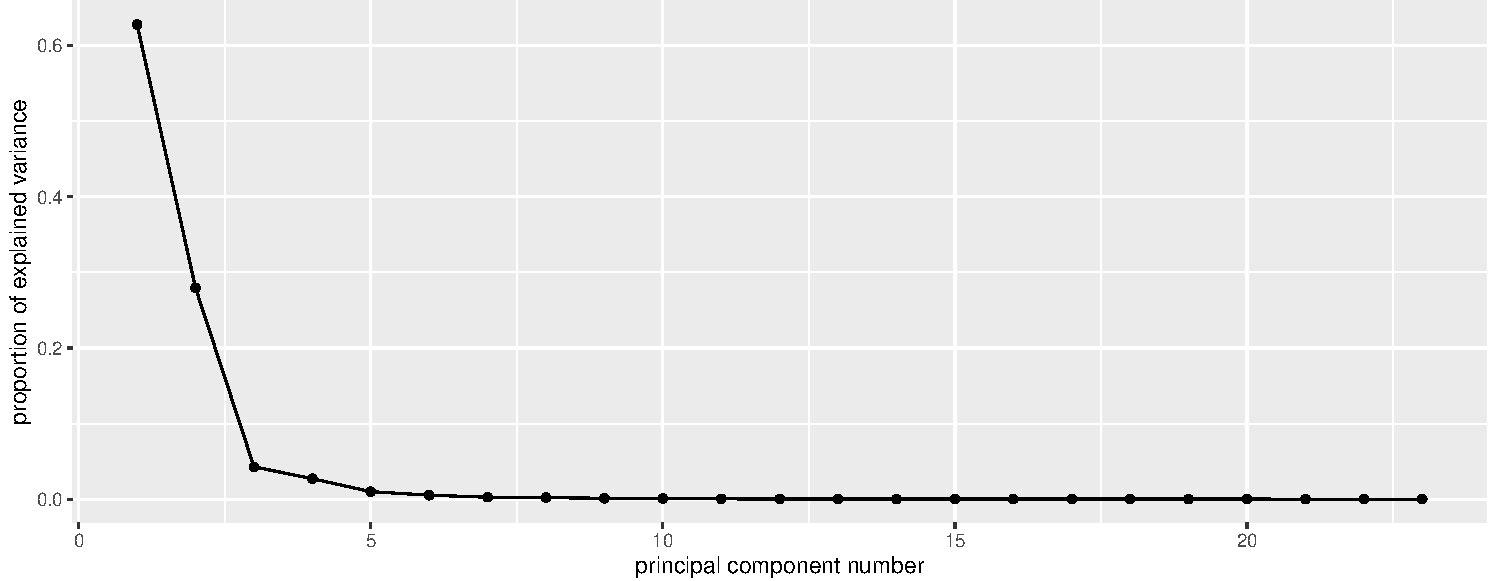
\includegraphics{unsupervised_learning_files/figure-beamer/unnamed-chunk-21-1.pdf}

\begin{Shaded}
\begin{Highlighting}[]
\KeywordTok{summary}\NormalTok{(pca.climate)}\OperatorTok{$}\NormalTok{importance[,}\DecValTok{1}\OperatorTok{:}\DecValTok{5}\NormalTok{]}
\end{Highlighting}
\end{Shaded}

\begin{verbatim}
##                             PC1      PC2       PC3       PC4       PC5
## Standard deviation     3.800932 2.535391 0.9915583 0.7882199 0.4761904
## Proportion of Variance 0.628130 0.279490 0.0427500 0.0270100 0.0098600
## Cumulative Proportion  0.628130 0.907620 0.9503700 0.9773800 0.9872400
\end{verbatim}

\end{frame}

\begin{frame}{Extensions and other considerations}
\protect\hypertarget{extensions-and-other-considerations-1}{}

\begin{itemize}
\tightlist
\item
  PCA assumes that the structure in the data is that of a normally
  distributed ellipsoidal point cloud, just one that's not lined up with
  the axes.
\item
  Other techniques allow for different structures in data. This is an
  area that is not far from the frontiers of statistics.
\item
  One area that has not been much investigated by ecologists and may
  have some low-hanging fruit is \emph{topological data analysis}.
\end{itemize}

\end{frame}

\begin{frame}{References}
\protect\hypertarget{references}{}

\hypertarget{refs}{}
\leavevmode\hypertarget{ref-islr}{}%
James, Gareth, Daniela Witten, Trevor Hastie, and Robert Tibshirani.
2013. \emph{An Introduction to Statistical Learning: With Applications
in R}. Springer.
\url{https://faculty.marshall.usc.edu/gareth-james/ISL/}.

\end{frame}

\end{document}
